\documentclass[
	xcolor={svgnames},
	hyperref={pagebackref,bookmarks},
	% aspectratio=169,
	aspectratio=43,
]{beamer}

\mode<presentation>
% %%%
% Author: Yihong Liu (https://liu-yihong.github.io/)
% Repository:
% License: GNU GPL v3.0
% This repository contains an unofficial LaTex beamer template for the University of Texas at Dallas.
% Copyright (c) 2022 Yihong Liu
%%%
\usepackage[utf8]{inputenc}
\usepackage{xcolor}
\usepackage{tikz}
% \usepackage{fontawesome5}
\usepackage{fontawesome}
% %%%
% Author: Yihong Liu (https://liu-yihong.github.io/)
% Repository:
% License: GNU GPL v3.0
% This repository contains an unofficial LaTex beamer template for the University of Texas at Dallas.
% Copyright (c) 2022 Yihong Liu
%%%
\usetheme{AnnArbor} % Dresden Berlin Madrid Singapore Frankfurt Montpellier
\usecolortheme{crane}
% https://www.cpt.univ-mrs.fr/~masson/latex/Beamer-appearance-cheat-sheet.pdf
\definecolor{utdorange}{RGB}{232,117,0}
\definecolor{utdgreen}{RGB}{18,71,52}
\definecolor{utdcyan}{RGB}{95,244,183}
\definecolor{utdcyangray}{RGB}{138,141,143}

\setbeamercolor*{structure}{bg=utdorange!40,fg=utdorange}

\setbeamercolor*{palette primary}{use=structure,fg=white,bg=structure.fg}
\setbeamercolor*{palette secondary}{use=structure,fg=white,bg=structure.fg!75}
\setbeamercolor*{palette tertiary}{use=structure,fg=white,bg=utdgreen}
\setbeamercolor*{palette quaternary}{fg=white,bg=structure.fg}

\setbeamercolor*{palette sidebar primary}{use=structure,fg=white,bg=structure.fg}
\setbeamercolor*{palette sidebar secondary}{use=structure,fg=white,bg=structure.fg!75}
\setbeamercolor*{palette sidebar tertiary}{use=structure,fg=white,bg=utdgreen}
\setbeamercolor*{palette sidebar quaternary}{fg=white,bg=structure.fg}

\setbeamercolor*{section in toc}{fg=black,bg=white}
% \setbeamercolor{alerted text}{use=structure,fg=utdcyan}
\setbeamercolor{block title alerted}{use=structure,bg=utdcyan}

\setbeamercolor{titlelike}{parent=palette primary,fg=white,bg=utdorange}
\setbeamercolor{frametitle}{bg=utdorange!85,fg=white}
% \setbeamercolor*{titlelike}{parent=palette primary}
\usetheme{CambridgeUS}
%%%
% Author: Yihong Liu (https://liu-yihong.github.io/)
% Repository:
% License: GNU GPL v3.0
% This repository contains an unofficial LaTex beamer template for the University of Texas at Dallas.
% Copyright (c) 2022 Yihong Liu
%%%
% https://tex.stackexchange.com/questions/443659/how-to-remove-date-from-footnote-of-madrid-theme-of-beamer-and-use-that-space-fo
\makeatletter
\setbeamertemplate{footline}{%
  \leavevmode%
  \hbox{%
    \begin{beamercolorbox}[wd=.15\paperwidth,ht=2.25ex,dp=1ex,center]{author in head/foot}{CS5150}%
%      \usebeamerfont{author in head/foot}\insertshortauthor\expandafter\ifblank\expandafter{\beamer@shortinstitute}{}{~~\insertshortinstitute}
    \end{beamercolorbox}%
    \begin{beamercolorbox}[wd=.77\paperwidth,ht=2.25ex,dp=1ex,center]{title in head/foot}%
      \usebeamerfont{title in head/foot}\insertshorttitle
    \end{beamercolorbox}%
  }%
  \begin{beamercolorbox}[wd=.08\paperwidth,ht=2.25ex,dp=1ex,right]{date in head/foot}%
    \usebeamerfont{date in head/foot}%
    \usebeamertemplate{page number in head/foot}%
    \hspace*{2ex}
  \end{beamercolorbox}
  \vskip0pt%
}
\makeatother
%gets rid of bottom navigation symbols
\setbeamertemplate{navigation symbols}{}
%gets rid of bottom navigation bars
% \setbeamertemplate{footline}[frame number]{}
%gets rid of footer
% \setbeamertemplate{footline}{}
%%%
% Author: Yihong Liu (https://liu-yihong.github.io/)
% Repository:
% License: GNU GPL v3.0
% This repository contains an unofficial LaTex beamer template for the University of Texas at Dallas.
% Copyright (c) 2022 Yihong Liu
%%%
\newcommand{\presentationtitle}{}
\newcommand{\presentationsubtitle}{}
\newcommand{\presenter}{}
\newcommand{\department}{}
\newcommand{\school}{}
\newcommand{\university}{}
\newcommand{\email}{}
\renewcommand{\presentationtitle}{Exact Exponential Algorithms}
\renewcommand{\presenter}{Taha Adeel Mohammed}
\renewcommand{\department}{Computer Science and Engineering}
\renewcommand{\school}{IITH}
\renewcommand{\university}{Indian Institute of Technology Hyderabad}
\renewcommand{\email}{\href{mailto:cs20btech11052@iith.ac.in}}
%%%
% Author: Yihong Liu (https://liu-yihong.github.io/)
% Repository:
% License: GNU GPL v3.0
% This repository contains an unofficial LaTex beamer template for the University of Texas at Dallas.
% Copyright (c) 2022 Yihong Liu
%%%
\hypersetup{
    pdfauthor={\presenter},%
    pdftitle={\presentationtitle - \presentationsubtitle},%
    pdfsubject={\department},%
    pdfkeywords={\department, \school, \university},%
    pdfproducer={LaTeX},%
    pdfcreator={pdfLaTeX},
    % bookmarks,
    bookmarksnumbered = true,
    bookmarksopen     = true,
    % pdfpagelabels     = true,
    pdfstartview={XYZ null null 1.2}
}

%% End of Template

\usepackage{blkarray}
\usepackage{amsmath}
\usepackage{amsfonts}
\usepackage{amssymb}
\usepackage{mathtools}
\usepackage{xcolor}
\usepackage{subfig}
\usepackage{chronology}

\title{\presentationtitle}
\subtitle{{- Under Dr. N.R. Aravind}}
\author{\presenter}
\institute[IITH]{
	\university\\
}
\date{\today}

\makeatletter
\makeatother

\begin{document}

\newcommand{\brak}[1]{\ensuremath{\left( #1 \right)}}
\newcommand{\sbrak}[1]{\ensuremath{\left[ #1 \right]}}
\newcommand{\Exp}[1]{\ensuremath{\mathbb{E} \left[ #1 \right]}}
\newcommand{\Var}[1]{\ensuremath{\text{Var} \left[ #1 \right]}}
\newcommand{\uar}{\stackrel{\$}{\leftarrow}}

% \setbeamercolor{alerted text}{fg=orange}

\begin{frame}
	\titlepage
\end{frame}

% \begin{frame}{Contents}
% 	\tableofcontents
% \end{frame}

% Slides:
% 1) Title Slide
% 2) Problem Statement
% 3) Matching Cut + Approaches to Matching Cut
% 4) 3-SAT + Matching Cut to 3-SAT
% 5) PPSZ Algorithm
% 6) PPSZ Analysis for Unique k-SAT
% 7-9) Hertli's Analysis for general k-SAT (2 Slides)
% 10) Matching Cut using P3 Double Dominating Set

\section{Problem Statement}
\begin{frame}{Problem Statement}
	\begin{itemize}
		\item<1-> Understand and analyse the different existing exponential algorithmic techniques. % Like branching algorithms, random walk algos, local search, dynamic programming, etc.
		\item<2-> Study the PPSZ algorithm for solving the \textsc{k-SAT} problem.
		\item<3-> Attempt to improve the current best known time complexity upper bound for the \textsc{Matching Cut} problem.
	\end{itemize}
\end{frame}

\section{Matching Cut Problem}
\begin{frame}{Matching Cut}
	\vspace*{-4mm}
	\begin{block}<1->{\textsc{Matching Cut} Problem}
		\vspace{-6mm}
		\begin{columns} % Text beside image
			\column{0.65\textwidth}
			\begin{itemize}
				\item Given a graph $G = (V, E)$.
				\item Decide whether it can be partitioned into two sets $A$ and $B$.
				\item $\forall\ v \in A$, $v$ has $\leq$ 1 neighbour in $B$ and vice versa.
			\end{itemize}
			\column{0.48\textwidth}
			\begin{figure}  \hspace{-15mm}
				\centering
				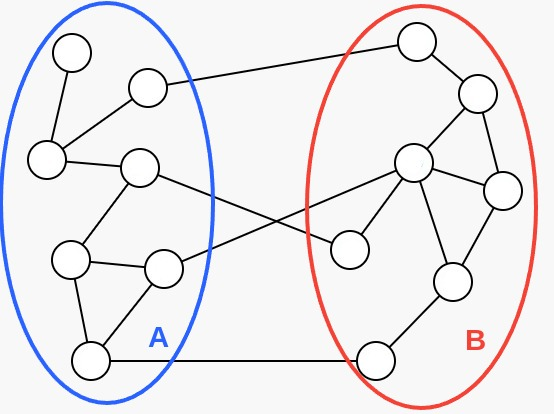
\includegraphics[width=0.65\textwidth]{images/matching-cut.jpeg}
			\end{figure}
		\end{columns}
	\end{block}
	\vspace*{-2mm}
	\begin{block}<2->{Approaches}
		\begin{itemize}
			\item \textsc{SAT}-free Branching Algorithm:\footnotemark[1]  $O^*(1.3803^n)$ 
			\item Reduction to \textsc{3-SAT}:\footnotemark[1]  $O^*(1.3071^n)$
			\item FPT algorithm for $d$-CUT:\footnotemark[2] $O^*(2^{O(k \log{k})})$ \hspace{3mm} ($k = $ max edge-cut size) 
		\end{itemize}
	\end{block}
	\setbeamerfont{footnote}{size=\scriptsize}
	\footnotetext[1]{Komusiewicz et al (2019). \textit{Matching Cut: Kernelization, Single-Exponential Time FPT, and Exact Exponential Algorithms}. 10.1016/j.dam.2019.12.010.}
	\footnotetext[2]{NR Aravind et al (2021). \textit{An FPT algorithm for Matching Cut and d-cut}. arXiv:2101.06998}
\end{frame}

\section{k-SAT}
\begin{frame}{k-SAT}
	\begin{block}{\textsc{k-SAT} Problem}
		Given a CNF formula with max $k$ literals per clause, decide if there exists an assignment that satisfies all clauses.
	\end{block}
	\begin{block}{\textsc{Matching Cut} to \textsc{3-SAT}}
		\begin{itemize}
			\item We add the constraint that for each $v \in V$, and its two neighbours $u_1, u_2$, they cannot be in different parts of the matching cut.
			\begin{align}
				\phi(G) = \bigwedge_{v \in V} \bigwedge_{u_1, u_2 \in N(v)} (v \vee \neg u_1 \vee \neg u_2) \wedge (\neg v \vee u_1 \vee u_2)
			\end{align} 
			\item $|Variables| = O(n)$, $|Clauses| = O(n^3)$
		\end{itemize}
	\end{block}
\end{frame}

\section{PPSZ Algorithm}
\begin{frame}{PPSZ Algorithm\footnotemark[3]}
	\vspace{-2mm}
	\underline{\textbf{Def$^\text{n}$}}: Let $F$ be a CNF formula and $D \in \mathbb{N}$. We say $F$ \textbf{D-implies} $u$ if $\exists\ G \subseteq F$ with $|G| \leq D$ that implies u.
	\vspace{-1mm}
	\begin{block}{Algorithm}
		\begin{itemize}
			\item  Randomly choose permutation $\pi$ of $vbl(\!F)$ and assignment $\!\beta \in \{0, 1\}^n$
			\item Process variables in $\pi$ order, setting each variable according to $\!\beta$, unless it is D-implied.
		\end{itemize}
	\end{block}
	\vspace{-2mm}
	\begin{block}{Timeline} \vspace{-3mm}
		\scriptsize
		\begin{chronology}[3]{1997}{2023}{\textwidth}
			\event{1999}{\tiny \underline{PPZ}: $O(1.5874^n)$}
			\event{2005}{$\frac{\text{\tiny PPSZ (Unique)}}{O(1.3070^n)}$}
			\event{2011}{$\frac{\text{\tiny Hertli's PPSZ (General)}}{O(1.3070^n)}$}
			\event{2014}{$\frac{\text{\tiny Hertli's Improvement}}{\approx 10^{-24} imp}$}
			\event{2017}{$\frac{\text{\tiny Scheder's Analysis}}{\approx 10^{-10} imp}$}
			\event{2019}{$\frac{\text{\tiny Thomas's Biased PPSZ}}{O(1.30699^n)}$}
			\event{2022}{$\frac{\text{\tiny Scheder's case work}}{O(1.30697^n)}$}
		\end{chronology}
	\end{block}
	\setbeamerfont{footnote}{size=\scriptsize}
	\footnotetext[3]{Ramamohan \textbf{P}aturi, \textbf{P}avel Pudlak, Michael E. \textbf{S}aks, and Francis \textbf{Z}ane. An improved exponential-time algorithm for k-SAT. J.ACM, 52(3):337{364, 2005}}
\end{frame}

\section{PPSZ Analysis for Unique k-SAT}
\begin{frame}{PPSZ Analysis for Unique k-SAT\footnotemark[4]}
	\vspace{-2.3mm}
	\underline{\textbf{Def$^\text{n}$}}: A variable $v$ is called \textbf{forced} if it is D-implied in $F$ by $\alpha$ (the unique satisfying assgn.) and variables before $v$ in $\pi$, else it is \textbf{guessed}. \vspace{-3.5mm}
	\begin{align}
		\underset{\beta, \pi}{\operatorname{Pr}}[\text{ppsz returns }\alpha] = \mathbb{E}_{\pi}[2^{-|\text{Guessed}(F, \alpha, \pi, D)|}] \geq 2^{-\sum\limits_x\operatorname{Pr}[x \text{ is guessed}]}
	\end{align}
	\vspace{-6mm}
	\begin{block}<2->{Critical Clause Tree}
		\vspace{-1.5mm}
		\begin{itemize}
			\setlength\itemsep{0.5mm}
			\item $T_x$ - Clause tree with var-label(root) $ = x$. Each node $u$ also has a clause-label($u$) and assignment $\beta(u)$ based on the tree construction.
			\item Represents how x can become D-implied in $F$.
			\item Reachable($T_x, \alpha, \pi$): Set of all nodes $u$ s.t.\! $\pi(v)\! \geq\! \alpha\ \forall\ v\! \in\!$ path($x, u$).
			\item \textbf{Clause Tree Lemma:} $|\text{Reachable}(T_x, \pi(x), \pi)| \leq D \Rightarrow x$ is forced.
		\end{itemize}
	\end{block}
	\vspace{-3mm}
	\begin{block}<3->{}
		Using above clause tree, distinct label lemma, extending $T'_x$ to $T_\infty$, and expectation calculations, we get:
		\vspace{-3mm}
		\begin{align}
			O^*(\text{ppsz}) = O^*(2^{(2 \ln 2 - 1)n}) = O^*(1.30704^n)
		\end{align}
	\end{block}
	
	\setbeamerfont{footnote}{size=\scriptsize}
	\footnotetext[4]{Paturi, Pudlak, Saks, and Zane. \textit{Chapter 6*: The PPSZ Algorithm}}
\end{frame}

\section{Hertli's Analysis for general k-SAT}
\subsection*{Introduction}
\begin{frame}{Hertli's Analysis for general k-SAT\footnotemark[5]}
	\vspace{-3.5mm}
	\begin{block}<1->{Definitions}
		\begin{itemize}
			\item $x$ is called a \textbf{frozen} variable if it has the same value in all satisfying assignments; \textbf{liquid} otherwise.
			\item $SL(F):$ Set of all satisfying literals. $|SL(F)| = |\text{frozen}| + 2|\text{liquid}|$
		\end{itemize}
	\end{block}
	\begin{block}<2->{Modified PPSZ Algorithm}
		Instead of strictly following $\pi$, after each step, all D-implied variables are immediately set.
	\end{block}
	\begin{block}<3->{Theorem-1}
		If $x$ is a frozen variable, then $p_{\text{guessed}}(F, x, \alpha, D) \leq S_k + \epsilon_k(D)$, where $S_k = \int_{0}^{1}\frac{t^{1/(k-1)} - t}{1 - t}$, and $\epsilon_k(D) \rightarrow 0$ as $D \rightarrow \infty$. \!\qquad\quad($S_3 = 2 \ln 2 - 1$)
	\end{block}
	\footnotetext[5]{Timon Hertli. \textit{3-SAT Faster and Simpler - Unique-SAT Bounds for PPSZ Hold in General.} IEEE, 2011.}
\end{frame}

\subsection*{Analysis using cost function}
\begin{frame}{Hertli's Analysis for general k-SAT}
	\vspace{-2.5mm}
	\begin{block}<1->{AssignSL(F)}
		\begin{itemize}
			\item Random process that generates a satisfying assignment.
			\item $\alpha = \{\}$; while $|\alpha| < n$: pick $\ell \in_R SL(F)$ and add it to $\alpha$; return $\alpha$;
			\item \underline{\textbf{Def$^\text{n}$}}: $p(F, \alpha) = $ Probability that AssignSL(F) returns $\alpha$.
			\vspace{-3mm}
			\begin{align}
				p(F, \alpha) = \frac{1}{|SL(F)|} \sum_{\ell \in \alpha} p(F^{[\ell]}, \alpha)
			\end{align}
		\end{itemize}
	\end{block}
	\vspace{-2mm}
	\begin{block}<2->{Cost Function}
		\begin{itemize}
			\item For variable $x$ in $F$, cost is defined as
			\vspace{-3mm}
			\begin{align}
				c(F, x) = \begin{cases}
					S_k & \text{if $x$ is liquid} \\
					\sum\limits_{\alpha \in sat(F)} p(F, \alpha) p_{\text{guessed}}(F, x, \alpha, D) & \text{if $x$ is frozen}
				\end{cases}
			\end{align}
			\vspace{-5.5mm}
			\item Cost of $F$ is defined as $c(F) = \sum_{x \in vbl(F)} c(F, x)$. \vspace{-2.5mm}
			\begin{align}
				\implies c(F) \leq n S_k \qquad\quad
			\end{align}
		\end{itemize}
	\end{block}
\end{frame}

\subsection{Success Probability}
\begin{frame}{Hertli's Analysis for general k-SAT}
	\begin{block}{Expectation of cost function (Theorem-2)}
		\vspace{-5mm}
		\begin{align}
			\mathbb{E}_\ell[c(F^{[\ell]})] \leq c(F) - |\text{liquid}|\frac{2 S_k}{|SL(F)|} - |\text{frozen}|\frac{S_k}{|SL(F)|}
		\end{align}
	\end{block}
	\begin{block}{\textbf{Success Probability}}
		\vspace{-6.5mm}
		\begin{align}
			p_{\text{success}}(F) \geq 2^{-c(F)}
		\end{align}
		\, \\ \vspace*{-5mm}
		% \vspace{-3mm}
		\textit{Proof by induction:} Base case trivial. \vspace{-2mm}
		\begin{align*}
			p_{\text{success}}(F) &= \frac{1}{2 n} \sum_{\ell \in SL(F)} p_{\text{success}}(F^{[\ell]})\ \geq \ \frac{1}{2 n} \sum_{\ell \in SL(F)} 2^{-c(F^{[\ell]})} \\
			&\geq \frac{|SL(F)|}{2n}\mathbb{E}_\ell[2^{-c(F^{[\ell]})}] \ \geq\ \frac{|SL(F)|}{2n}2^{-\mathbb{E}_\ell[c(F^ {[\ell]})]} \\
			\implies p_{\text{success}}(F) &\geq 2^{\log \frac{|SL(F)|}{2n} - \mathbb{E}_\ell[c(F^ {[\ell]})]} \ \geq \ 2^{-c(F)}
		\end{align*}
		\vspace{-15mm}
		\begin{flushright}
			$\qedsymbol$
		\end{flushright}
	\end{block}
\end{frame}

\section{Matching Cut using $P_3$ Double Dominating Set}
\begin{frame}{Matching Cut using $P_3$ Double Dominating Set}
	\vspace{-2mm}
	\begin{block}<1->{$P_3$ Double Dominating Set}
		\begin{itemize}
			\item Let $S \subseteq V$ s.t. every $P_3$ of $G[V \setminus S]$ has a vertex with atleast 2 neighbours in $S$.
			\item \textbf{Proposition:} Let $G$ be a $n$-vertex graph without leaves or adjacent degree-2 vertices. Then $\exists \ S$ s.t. $|S| \leq \left \lceil{\frac{2n}{5}}\right \rceil 
			$, which can be found quickly.
		\end{itemize}
	\end{block}
	\vspace{-2mm}
	\begin{block}<2->{Algorithm}
		\vspace{-2mm}
		Brute-force vertices in $S$ in $O(2^{|S|})$ and check for Matching Cut by reduction to 2-SAT:
		\begin{enumerate}
			\item For $v \in S$, add clause $(x_v)$ or $(\neg x_v)$ based on $v \in A$ or $v \in B$.
			\item For $v \in V \setminus S$ and $u_1, u_2 \in N(v)$,
			\begin{itemize}
				\item If $x_{u_1} = x_{u_2}$, then $x_v = x_{u_1}$, i.e. add ($x_v$) or ($\neg x_v$) appropriately.
				\item Else if $x_{u_1} = x_{u_2}$, then $\forall\ u \in N(v) \setminus \{u_1, u_2\}$, we have the condition $x_u = x_v$, i.e. add $(x_v \vee \neg x_u) \wedge (\neg x_v \vee x_u)$. 
			\end{itemize}
		\end{enumerate}
	\end{block}
\end{frame}

\begin{frame}[noframenumbering]
	\begin{center}
		\huge Thank You! 
	\end{center}
\end{frame}  

\end{document}


% Speaker notes:
% 1) Good afternoon everyone. I am Taha Adeel Mohammed. The project I worked on was on Exact Exponential Algorithms under Professor N.R. Aravind. 

% 2) The goal of the project was to understand the different existing exponential algorithmic techniques like branching, and to study the PPSZ algorithm for the k-SAT problem. Then using these techniques and insights from the PPSZ algorithm, try to improve the current best time complexity bound for the Matching Cut problem.

% 3) So the matching cut problem asks whether you can partition a graph into sets A and B such that any vertex has atmost one neighbour in the other set. The approaches to solve it include a branching algorithm, reduction to 3-SAT, and parametrized algos, with the best one being Reduction to 3-SAT.

% 4) To reduce Matching Cut to 3-SAT, we add constraints that for each vertex v and its neighbours u1, u2, both neighbours cannot be in the other set, giving rise to the condition (v or not u1 or not u2) and (not v or u1 or u2).

% 5) Now we look at the PPSZ Algorithm, which is the current fastest algorithm for solving the k-SAT problem. It is a simple algorithm, with its runtime analysis being the hard part. So we say that a CNF formula F D-implies a variable u if there exists a subset of atmost D clauses that imply u. The algorithm randomly chooses a permutation of variables and an assignment \beta, and processes the variables in that order, setting them unless they are D-implied. The algorithm has been extensively studied, with the recent improvements being very minute, tho still meaningful.

% 6) We first take a quick look at the analysis for when the k-SAT has a unique satisying assignment \alpha. We define a variable to be forced if it is D-implied by the unique assignment, and guessed otherwise. The probability that ppsz returns the correct assignment is that all guessed variables are set correctly, as shown by (2). The authors introduce the concept of a critical clause tree, which represents how a variable can become D-implied in F. The clause tree lemma states that if the number of reachable nodes in the tree is atmost D, then the variable is forced. For the analysis, the clause tree labels are then made all distinct, and then it is extended to an infinite tree to help bound the probability of guessing a variable. The final analysis gives a runtime of O*(2^{(2 ln 2 - 1)n}) = O*(1.30704^n). 

% 7) Extending the anaysis from unique k-SAT to general k-SAT remained an open problem for 13 years, before Timon Hertli solved it in 2011. He introduced the concept of frozen and liquid variables, frozen variables having the same value in all satifying \alphas, and modified the PPSZ algorithm to immediately set D-implied variables. For frozen variables, the probability of guessing them is given by S_k, the constant from the unique k-SAT case, and the proof for this theorem is based on the critical clause tree.

% 8) Hertli defines a random process AssignSL to generate satisfying assignments by randomly picking satisfying literals. p(F, \alpha) is defined as the probability that AssignSL returns \alpha, and it satifies the recursive relation given by (4). We then define a cost function for variables in F, and the cost of F as the sum of costs of all variables. The cost of F is bounded by nS_k, since if a variable is liquid, by definition cost is S_k, and if it is frozen, using theorem 1 and the fact that prob < 1, the bound holds again.

% 9) We now claim the success probability is atleast 2^{-c(F)}, and since c(F) is bounded by nS_k, we would get the equivalent result for general k-SAT as well. The proof is by induction, with the base case being trivially true. We have probability of success of F as the average of success after randomly picking a literal. Then using the induction hypothesis, we 2^-c(F) into the summation. Then replacing summation with n times expectation and using Jensen's inequality, we get probability of success is atleast 2 power log SL by 2n - expectation of the cost function. Using theorem 2, it can be shown that this is atleast 2 power -c(F), and hence the claim holds.

% 10) Another approach we tried for solving Matching Cut was using P3 double dominating sets, which basically means that for every path with length 3 not in the dominating set S, the path has a vertex with atleast 2 neighbours in S. We proposed that the minimum size of S can be bound by ceil(2n/5). Assuming we have such a set, to solve Matching Cut, we brute force all vertices in S in 2 power |S| time and check for a matching cut by reducing it to 2-SAT. For each vertex in S, we add a clause based on which set it belongs to. For vertices not in S, if it has 2 neighbours in the same set, then it also has to belong to that set. And if its neighbours are in different sets, then its other neighbours have to be in the same set as it. This can be represented as the 2-SAT boolean clause (x_v or not x_u) and (not x_v or x_u). Finding a valid S quickly proved challenging for this approach.

% 11) Thank you for listening.